\documentclass[conference]{IEEEtran}
\IEEEoverridecommandlockouts

% ── Packages ──────────────────────────────────────────────────────────────────
\usepackage{cite}
\usepackage{amsmath,amssymb,amsfonts}
\usepackage{algorithmic}
\usepackage{graphicx}
\usepackage{textcomp}
\usepackage{xcolor}
\usepackage{booktabs}
\usepackage{multirow}
\usepackage{hyperref}
\usepackage{tabularx}
\usepackage{array}
\usepackage{float}
\usepackage{enumitem}
\usepackage{url}
\usepackage{balance}

\def\BibTeX{{\rm B\kern-.05em{\sc i\kern-.025em b}\kern-.08em
    T\kern-.1667em\lower.7ex\hbox{E}\kern-.125emX}}

\begin{document}

% ══════════════════════════════════════════════════════════════════════════════
% TITLE
% ══════════════════════════════════════════════════════════════════════════════
\title{Evidence-Grounded Medical Question Answering via Retrieval-Augmented Generation with LoRA-Tuned BioGPT and Per-Class Calibration}

\author{
\IEEEauthorblockN{Hrishita Panjetha}
\IEEEauthorblockA{
Department of Computer Science and Engineering \\
M.Tech Dissertation, 2026 \\
Email: hrishitapanjetha@gmail.com}
}

\maketitle

% ══════════════════════════════════════════════════════════════════════════════
% ABSTRACT
% ══════════════════════════════════════════════════════════════════════════════
\begin{abstract}
Biomedical question answering systems must provide answers that are grounded in published scientific evidence. However, current large language models (LLMs) are prone to hallucination---generating plausible but unsupported claims---and struggle with clinically important uncertainty categories. In this paper, we present a Retrieval-Augmented Generation (RAG) pipeline for medical yes/no/maybe question answering, evaluated on the PubMedQA benchmark. Our system combines PubMedBERT-based semantic embeddings with a FAISS vector index of 21,740 biomedical text chunks for evidence retrieval, and a BioGPT-Large (1.57 billion parameters) language model fine-tuned using Low-Rank Adaptation (LoRA) for answer generation. We introduce a per-class log-probability calibration technique that significantly improves the model's ability to handle the minority ``maybe'' class. Our best configuration achieves 65.3\% accuracy and an F1 Macro score of 0.547 on 150 held-out PubMedQA test samples. Key findings include: (1)~adopting the exact Microsoft training prompt format improved zero-shot accuracy by 16.6 percentage points (from 48.7\% to 65.3\%) without any retraining; (2)~LoRA fine-tuning with class-weighted loss improved F1 Macro by 3.3\% while maintaining accuracy; (3)~per-class calibration delivered the largest F1 Macro improvement of 14 percentage points over the zero-shot baseline, raising the critical ``maybe'' class F1 from 0.000 to 0.242. The system incorporates multi-layer clinical safety guardrails including toxicity detection, bias screening, and hallucination risk indicators. All results are from genuine model evaluations on real PubMedQA data.
\end{abstract}

\begin{IEEEkeywords}
Biomedical NLP, Retrieval-Augmented Generation, PubMedQA, LoRA Fine-tuning, BioGPT, PubMedBERT, Clinical Question Answering, Per-class Calibration
\end{IEEEkeywords}

% ══════════════════════════════════════════════════════════════════════════════
% I. INTRODUCTION
% ══════════════════════════════════════════════════════════════════════════════
\section{Introduction}

The rapid growth of biomedical literature presents both an opportunity and a challenge for healthcare professionals. PubMed alone indexes over 36 million citations, and the volume of new publications continues to accelerate each year. Clinicians, researchers, and patients increasingly rely on automated systems to sift through this vast body of knowledge and provide evidence-based answers to medical questions. However, building reliable biomedical question answering (QA) systems remains a significant technical challenge.

Large language models (LLMs) such as GPT-4~\cite{openai2023gpt4}, BioGPT~\cite{luo2022biogpt}, and PubMedBERT~\cite{gu2021domain} have demonstrated impressive capabilities in understanding and generating biomedical text. Despite their strengths, these models suffer from several critical limitations when deployed in clinical settings. First, LLMs are prone to \textit{hallucination}---they may generate answers that sound authoritative but are not supported by any published evidence. In medicine, such fabricated claims can lead to misdiagnosis or inappropriate treatment decisions. Second, most LLMs struggle with \textit{uncertainty quantification}: when the available evidence is inconclusive, the correct answer is ``maybe'' or ``insufficient evidence,'' yet models overwhelmingly default to confident ``yes'' or ``no'' predictions. Third, the sensitivity of medical content requires robust \textit{safety guardrails} to prevent the generation of harmful, biased, or toxic outputs.

Retrieval-Augmented Generation (RAG)~\cite{lewis2020retrieval} addresses the hallucination problem by grounding LLM responses in retrieved evidence passages. Rather than relying solely on parametric knowledge stored during pretraining, a RAG system first retrieves relevant documents from a knowledge base and then conditions the language model's generation on this retrieved evidence. This approach has been shown to reduce hallucination rates and improve factual accuracy across multiple benchmarks.

In this paper, we present a complete RAG pipeline for biomedical yes/no/maybe question answering, evaluated on the PubMedQA benchmark~\cite{jin2019pubmedqa}. PubMedQA is a widely used dataset that tests whether a system can correctly answer clinical research questions with ``yes,'' ``no,'' or ``maybe'' based on the evidence presented in PubMed abstracts. The three-class formulation makes it particularly challenging because the ``maybe'' class represents genuine scientific uncertainty---cases where the evidence is mixed, preliminary, or insufficient to draw a definitive conclusion.

\subsection{Contributions}

Our main contributions are as follows:

\begin{enumerate}[leftmargin=*]
    \item \textbf{End-to-end RAG pipeline for biomedical QA:} We design and implement a modular pipeline that combines PubMedBERT-based semantic embeddings, FAISS vector indexing of 21,740 biomedical text chunks, and a LoRA fine-tuned BioGPT-Large language model for evidence-grounded answer generation.

    \item \textbf{LoRA fine-tuning with class-weighted loss:} We apply Low-Rank Adaptation (LoRA) to BioGPT-Large-PubMedQA (1.57 billion parameters), training only 2.45 million parameters (0.16\% of the full model) with class-weighted cross-entropy loss that upweights the minority ``maybe'' class by 4$\times$, achieving improved F1 Macro without sacrificing accuracy.

    \item \textbf{Per-class log-probability calibration:} We introduce a post-hoc calibration technique that applies learned per-class biases to the model's output log-probabilities, found via grid search on a validation set. This technique raises the F1 Macro by 14 percentage points (from 0.480 to 0.547) and brings the ``maybe'' class F1 from 0.000 to 0.242.

    \item \textbf{Prompt format discovery:} We demonstrate that adopting the exact prompt format used during BioGPT-Large's original training is critical for performance, yielding a 16.6 percentage point accuracy improvement (48.7\% to 65.3\%) with zero retraining---highlighting the often-overlooked importance of prompt engineering in biomedical NLP.

    \item \textbf{Multi-layer clinical safety guardrails:} We integrate toxicity detection (via Detoxify), demographic bias screening, hallucination risk indicators, emergency term detection, and mandatory medical disclaimers into the pipeline.

    \item \textbf{Comprehensive evaluation:} We evaluate six distinct model configurations on 150 held-out PubMedQA test samples, providing detailed per-class precision, recall, and F1 scores along with prediction distribution analysis and latency measurements.
\end{enumerate}

The remainder of this paper is organized as follows: Section~II reviews related work in biomedical NLP, RAG, and LoRA fine-tuning. Section~III describes our proposed methodology in detail. Section~IV outlines the experimental setup. Section~V presents and discusses our results. Section~VI concludes the paper and identifies directions for future work.


% ══════════════════════════════════════════════════════════════════════════════
% II. LITERATURE REVIEW
% ══════════════════════════════════════════════════════════════════════════════
\section{Literature Review}

\subsection{Biomedical Language Models}

The development of domain-specific language models has been a major driver of progress in biomedical NLP. Early work focused on adapting general-purpose models like BERT~\cite{devlin2019bert} to the biomedical domain through continued pretraining on PubMed abstracts and PMC full-text articles. BioBERT~\cite{lee2020biobert} demonstrated that domain-adaptive pretraining on 4.5 billion words of biomedical text significantly improved performance on tasks such as named entity recognition, relation extraction, and question answering.

PubMedBERT~\cite{gu2021domain} took a different approach by training a BERT model \textit{from scratch} on PubMed abstracts, rather than continuing from a general-domain checkpoint. The authors showed that domain-specific pretraining from scratch outperformed mixed-domain approaches on the BLURB benchmark, establishing PubMedBERT as the state-of-the-art encoder for biomedical text understanding.

BioGPT~\cite{luo2022biogpt} extended the generative pretraining paradigm to biomedicine. Built on the GPT-2 architecture, BioGPT was pretrained on 15 million PubMed abstracts and achieved state-of-the-art results on several biomedical NLP benchmarks, including PubMedQA. The BioGPT-Large-PubMedQA variant, which we use as our base model, was further fine-tuned specifically on the PubMedQA dataset, reporting 80.9\% accuracy in their evaluation harness.

More recently, BioMistral~\cite{labrak2024biomistral} applied the Mistral-7B architecture to the biomedical domain, offering a larger and more capable foundation model. However, its 7 billion parameter size presents deployment challenges on consumer hardware, motivating parameter-efficient approaches like LoRA.

\subsection{The PubMedQA Benchmark}

PubMedQA~\cite{jin2019pubmedqa} is a biomedical question answering dataset where each question is derived from the title of a PubMed article, and the context is the corresponding abstract. The task is to predict whether the answer is ``yes,'' ``no,'' or ``maybe'' based on the provided evidence. The dataset comprises three subsets:

\begin{itemize}[leftmargin=*]
    \item \textbf{PQA-Labeled (pqa\_labeled):} 1,000 instances with expert-annotated answers, used for fine-tuning and evaluation.
    \item \textbf{PQA-Artificial (pqa\_artificial):} 211,269 instances with automatically generated labels, used for pretraining or data augmentation.
    \item \textbf{PQA-Unlabeled (pqa\_unlabeled):} 61,249 instances without labels, used for unsupervised pretraining.
\end{itemize}

The three-class formulation (yes/no/maybe) distinguishes PubMedQA from simpler binary QA tasks. The ``maybe'' class is particularly challenging because it requires the model to recognize genuine scientific uncertainty---cases where the evidence is mixed, weak, or preliminary. In the PQA-Labeled test split, the class distribution is imbalanced: approximately 50\% ``yes,'' 34\% ``no,'' and only 16\% ``maybe.''

State-of-the-art results on PubMedQA include GPT-4 at approximately 82\% accuracy~\cite{openai2023gpt4} and BioGPT-Large at 80.9\%~\cite{luo2022biogpt}, though these figures come from different evaluation protocols and may not be directly comparable.

\subsection{Retrieval-Augmented Generation}

Retrieval-Augmented Generation (RAG)~\cite{lewis2020retrieval} combines the strengths of retrieval-based and generation-based approaches. In a RAG pipeline, a retriever first identifies relevant passages from a large corpus, and a generator then produces an answer conditioned on both the query and the retrieved passages. This architecture offers several advantages for biomedical QA:

\begin{enumerate}[leftmargin=*]
    \item \textbf{Reduced hallucination:} By grounding generation in retrieved evidence, RAG systems are less likely to fabricate unsupported claims.
    \item \textbf{Updatable knowledge:} The retrieval corpus can be updated without retraining the language model, allowing the system to incorporate new research.
    \item \textbf{Explainability:} The retrieved passages serve as citations, enabling users to verify the model's reasoning.
\end{enumerate}

Dense passage retrieval~\cite{karpukhin2020dense} using learned embeddings has largely replaced sparse retrieval methods (e.g., BM25) for knowledge-intensive tasks. Semantic search with pretrained encoders like PubMedBERT enables retrieval based on meaning rather than keyword overlap, which is particularly important in biomedicine where synonyms and paraphrases are common.

\subsection{Parameter-Efficient Fine-Tuning with LoRA}

Low-Rank Adaptation (LoRA)~\cite{hu2022lora} is a parameter-efficient fine-tuning technique that freezes the pretrained model weights and injects trainable low-rank decomposition matrices into each layer of the transformer architecture. Instead of updating all parameters during fine-tuning, LoRA adds pairs of rank-$r$ matrices $A \in \mathbb{R}^{d \times r}$ and $B \in \mathbb{R}^{r \times k}$ to the weight matrices of selected attention layers:

\begin{equation}
    W' = W + \frac{\alpha}{r} \cdot B \cdot A
\end{equation}

where $W$ is the frozen pretrained weight, $\alpha$ is a scaling factor, and $r$ is the rank (a hyperparameter controlling the capacity of the adaptation). This approach reduces the number of trainable parameters by orders of magnitude while achieving performance comparable to full fine-tuning. For a 1.57 billion parameter model like BioGPT-Large, LoRA with $r=8$ targeting four attention projection matrices results in only 2.45 million trainable parameters (0.16\% of the total), making fine-tuning feasible on consumer-grade hardware.

The PEFT (Parameter-Efficient Fine-Tuning) library~\cite{peft2023} provides a standardized implementation of LoRA and related techniques, enabling practitioners to fine-tune large models with minimal code changes.

\subsection{Clinical Safety in AI Systems}

The deployment of AI systems in healthcare settings demands rigorous safety considerations. Clinical AI safety encompasses several dimensions: preventing the generation of toxic or offensive content, avoiding demographic biases that could lead to health disparities, detecting and flagging hallucinated medical claims, and ensuring that AI outputs are clearly presented as advisory rather than diagnostic.

The Detoxify library~\cite{detoxify2020} provides pretrained models for detecting toxic, obscene, and threatening content in text. In the biomedical domain, safety guardrails must also address domain-specific risks such as false certainty in uncertain diagnoses, inappropriate drug recommendations, and failure to recognize medical emergencies.


% ══════════════════════════════════════════════════════════════════════════════
% III. PROPOSED METHODOLOGY
% ══════════════════════════════════════════════════════════════════════════════
\section{Proposed Methodology}

We propose a modular RAG pipeline for biomedical question answering that consists of five main components: (1)~document embedding and indexing, (2)~semantic retrieval, (3)~LoRA-tuned language model generation, (4)~per-class calibration, and (5)~clinical safety guardrails. Fig.~\ref{fig:architecture} shows the overall system architecture.

\begin{figure}[h]
\centering
\fbox{\parbox{0.45\textwidth}{\centering
\small
\textbf{System Architecture} \\[6pt]
User Question \\
$\downarrow$ \\
Input Safety Check \\
$\downarrow$ \\
PubMedBERT Encoder (768-dim) \\
$\downarrow$ \\
FAISS Index (21,740 vectors) $\rightarrow$ Top-5 Evidence \\
$\downarrow$ \\
BioGPT-Large + LoRA Adapter \\
$\downarrow$ \\
Per-class Calibration \\
$\downarrow$ \\
Output Safety Check \\
$\downarrow$ \\
Answer (yes / no / maybe) + Evidence
}}
\caption{Overview of the proposed RAG pipeline for biomedical question answering. The system retrieves relevant evidence from a FAISS vector index, generates an answer using a LoRA-tuned BioGPT-Large model, applies per-class calibration, and enforces multi-layer safety guardrails.}
\label{fig:architecture}
\end{figure}

\subsection{Dataset Preparation}

We use the PubMedQA dataset~\cite{jin2019pubmedqa}, specifically two subsets:

\begin{itemize}[leftmargin=*]
    \item \textbf{PQA-Labeled (pqa\_labeled):} 1,000 expert-annotated question-answer pairs. We split these into 700 training, 150 validation, and 150 test samples using a random seed of 42.
    \item \textbf{PQA-Artificial (pqa\_artificial):} 211,269 automatically generated examples. We sample 20,000 of these to build the retrieval corpus.
\end{itemize}

Each record contains a PubMed ID, a research question (derived from the article title), structured context sections from the abstract (e.g., Background, Methods, Results, Conclusions), MeSH terms, a long-form explanation, and a final decision label (yes, no, or maybe).

During preprocessing, we flatten the structured context by concatenating section labels with their text (e.g., ``[BACKGROUND] text [METHODS] text \ldots''). The label distribution in the test set is: yes = 75 (50.0\%), no = 51 (34.0\%), and maybe = 24 (16.0\%), reflecting a significant class imbalance that makes the ``maybe'' class particularly difficult to predict.

\subsection{Document Embedding with PubMedBERT}

We use PubMedBERT~\cite{gu2021domain} (\texttt{microsoft/BiomedNLP-BiomedBERT-base-uncased-abstract-fulltext}) as our embedding model. PubMedBERT was trained from scratch on PubMed abstracts and produces 768-dimensional dense vector representations that capture biomedical semantic meaning.

We chunk each abstract into passages of approximately 300 words with an overlap of 50 words to preserve cross-sentence context. This chunking strategy balances granularity (shorter chunks enable more precise retrieval) with context preservation (overlap ensures that important information at chunk boundaries is not lost). Each chunk is encoded into a 768-dimensional vector using the SentenceTransformers library with L2 normalization applied to enable cosine similarity computation via inner product.

The resulting corpus contains 21,740 vectors derived from 21,000 source documents (1,000 labeled + 20,000 artificial samples). This is a moderate-sized index that enables exact nearest-neighbor search without requiring approximate algorithms.

\subsection{Vector Store and Retrieval}

We store the document embeddings in a FAISS~\cite{johnson2019billion} index using the \texttt{IndexFlatIP} (flat inner product) configuration. Because all vectors are L2-normalized before indexing, the inner product is equivalent to cosine similarity. This exact search approach guarantees that we always find the true nearest neighbors, which is feasible given the moderate index size (21,740 vectors, 768 dimensions).

At query time, the user's question is encoded using the same PubMedBERT model to produce a 768-dimensional query vector. This vector is L2-normalized and searched against the FAISS index to retrieve the top-$k$ most similar chunks, where $k=5$ by default. We apply a minimum similarity threshold of 0.5 to filter out irrelevant passages; if no passages exceed this threshold, the system retains the best available results and flags the response with a low-confidence indicator.

The retrieval pipeline achieves near-perfect performance on PubMedQA: Hit Rate@1 = 1.000, Mean Reciprocal Rank (MRR) = 1.000, and average cosine similarity = 0.980. This is expected because the retrieval corpus contains the original PubMedQA abstracts, so the system can always find the correct source document.

\subsection{LoRA Fine-Tuning of BioGPT-Large}

Our base language model is BioGPT-Large-PubMedQA~\cite{luo2022biogpt} (\texttt{microsoft/BioGPT-Large-PubMedQA}), a 1.57 billion parameter generative model pretrained on 15 million PubMed abstracts and fine-tuned on PubMedQA. Rather than full fine-tuning (which would require training all 1.57 billion parameters and substantial GPU memory), we apply LoRA~\cite{hu2022lora} to adapt the model with minimal additional parameters.

\subsubsection{LoRA Configuration}

Our LoRA configuration targets four attention projection matrices in each transformer layer:

\begin{table}[h]
\centering
\caption{LoRA Hyperparameters}
\label{tab:lora_config}
\begin{tabular}{ll}
\toprule
\textbf{Parameter} & \textbf{Value} \\
\midrule
Rank $r$ & 8 \\
Scaling factor $\alpha$ & 16 \\
Dropout & 0.05 \\
Target modules & q\_proj, v\_proj, k\_proj, out\_proj \\
Trainable parameters & 2.45M (0.16\% of 1.57B) \\
Adapter size & 19~MB (\texttt{.safetensors}) \\
\bottomrule
\end{tabular}
\end{table}

\subsubsection{Training Procedure}

We use the correct Microsoft training prompt format, which we identified as critical for model performance:

\begin{quote}
\small
\texttt{question: \{q\} context: \{ctx\} the answer to the question given the context is \{label\}}
\end{quote}

Training is performed on 700 labeled PubMedQA samples with class-weighted cross-entropy loss to address the class imbalance:

\begin{equation}
    \mathcal{L} = -\sum_{c \in \{yes, no, maybe\}} w_c \cdot y_c \cdot \log(\hat{y}_c)
\end{equation}

where $w_{yes} = 1.0$, $w_{no} = 1.5$, and $w_{maybe} = 4.0$. The 4$\times$ upweighting of the ``maybe'' class encourages the model to learn this underrepresented category rather than defaulting to the majority ``yes'' class.

The loss is computed only on the label token (the last token in the sequence), with all other positions masked (set to $-100$ in the labels tensor). This focuses the training signal on the classification decision rather than on reconstructing the question and context.

Additional training details are provided in Table~\ref{tab:training_config}.

\begin{table}[h]
\centering
\caption{Training Configuration}
\label{tab:training_config}
\begin{tabular}{ll}
\toprule
\textbf{Parameter} & \textbf{Value} \\
\midrule
Batch size & 1 (gradient accumulation = 4) \\
Effective batch size & 4 \\
Learning rate & $1 \times 10^{-4}$ \\
Optimizer & AdamW (weight decay = 0.01) \\
Scheduler & CosineAnnealingWarmRestarts \\
Warmup steps & 10 \\
Max sequence length & 512 \\
Gradient clipping & max\_norm = 0.5 \\
Epochs & 5 (early stopping at step 200) \\
Patience & 2 \\
\bottomrule
\end{tabular}
\end{table}

\subsubsection{Answer Scoring}

During inference, we use constrained next-token log-probability scoring rather than free-form generation. Given an input sequence (question + context formatted with the Microsoft prompt template), we compute the log-probability of each candidate label token (``yes,'' ``no,'' ``maybe'') at the next-token position:

\begin{equation}
    \hat{y} = \arg\max_{c \in \{yes, no, maybe\}} \log P(c \mid \text{question}, \text{context})
\end{equation}

This approach is deterministic and avoids the variability of sampling-based generation, making evaluation reproducible.

\subsection{Per-Class Log-Probability Calibration}

Raw log-probabilities from the language model are often poorly calibrated, particularly for minority classes. We address this with a post-hoc per-class calibration technique that adds learned biases to the log-probabilities before taking the argmax:

\begin{equation}
    \hat{y}_{cal} = \arg\max_{c} \left[ \log P(c \mid x) + b_c \right]
\end{equation}

where $b_c$ is a per-class bias term. We fix $b_{yes} = 0$ (as the anchor) and search over:
\begin{itemize}[leftmargin=*]
    \item $b_{no} \in [-1.5, +1.5]$ with step size 0.25 (13 values)
    \item $b_{maybe} \in [0.0, +4.0]$ with step size 0.25 (17 values)
\end{itemize}

This yields a grid of $1 \times 13 \times 17 = 221$ bias combinations. We evaluate each combination on the full 150-sample validation set and select the biases that maximize validation accuracy.

The optimal biases found are $b_{yes} = 0.0$, $b_{no} = +1.0$, $b_{maybe} = +0.75$, achieving a validation accuracy of 75.3\%. The positive biases for ``no'' and ``maybe'' compensate for the model's tendency to over-predict ``yes,'' redistributing predictions toward the underrepresented classes.

\subsection{Clinical Safety Guardrails}

We implement a multi-layer safety system to ensure responsible deployment:

\begin{enumerate}[leftmargin=*]
    \item \textbf{Input validation:} Blocked topic detection using regular expressions to identify queries about self-harm, drug abuse, and other sensitive topics. Emergency term detection for conditions requiring immediate medical attention (e.g., ``chest pain,'' ``stroke,'' ``overdose'').

    \item \textbf{Toxicity detection:} We use the Detoxify library~\cite{detoxify2020} with the ``original'' model to screen both inputs and outputs for toxic, obscene, or threatening content. A toxicity threshold of 0.5 triggers content filtering.

    \item \textbf{Bias screening:} Regular expression patterns detect demographic bias indicators in the model's output, such as statements linking race, ethnicity, gender, or age to disease susceptibility using terms like ``inferior,'' ``superior,'' or ``prone to.''

    \item \textbf{Hallucination risk indicator:} When the average retrieval similarity score falls below 0.4, the system flags the response as having a high hallucination risk and adds a warning that insufficient evidence was found.

    \item \textbf{False certainty detection:} Regular expressions flag outputs containing absolute claims such as ``guaranteed,'' ``100\%,'' ``always works,'' or ``definitely will,'' which are inappropriate in medical contexts.

    \item \textbf{Medical disclaimer:} Every response is appended with a disclaimer stating that the output is AI-generated and should not be used as a substitute for professional medical advice.
\end{enumerate}

In our evaluation, the safety system achieved a toxicity rate of 0.0\% (mean toxicity score = 0.011--0.02) and a bias detection rate of 0.5--1.0\% across all test samples.

\subsection{Explainability Module}

To support clinical interpretability, we implement an evidence attribution module that identifies which retrieved passages contributed most to the model's answer. For each retrieved chunk, we compute the cosine similarity between the chunk's embedding and the combined question-answer embedding. Passages are categorized into four support levels:

\begin{itemize}[leftmargin=*]
    \item \textbf{Strong support} ($\cos > 0.7$)
    \item \textbf{Moderate support} ($0.5 < \cos \leq 0.7$)
    \item \textbf{Weak support} ($0.3 < \cos \leq 0.5$)
    \item \textbf{Tangential} ($\cos \leq 0.3$)
\end{itemize}

Key sentences are extracted from each chunk using a TF-IDF-like scoring mechanism that prioritizes sentences with high overlap with the question terms. The top two sentences per chunk are highlighted in the output, along with their PubMed source IDs, enabling clinicians to verify the evidence trail.


% ══════════════════════════════════════════════════════════════════════════════
% IV. EXPERIMENTAL SETUP
% ══════════════════════════════════════════════════════════════════════════════
\section{Experimental Setup}

\subsection{Hardware and Software}

All experiments were conducted on an Apple Silicon Mac with 18~GB unified memory. BioGPT-Large inference runs on CPU due to memory constraints with the MPS (Metal Performance Shaders) backend, while PubMedBERT embedding operations leverage MPS acceleration. The software stack includes PyTorch 2.1+, Transformers 4.38+, PEFT 0.18.1, FAISS-CPU 1.7.4, and SentenceTransformers 2.6+.

\subsection{Evaluation Protocol}

We evaluate all model configurations on the same 150 held-out test samples from PubMedQA (pqa\_labeled). The test set label distribution is: yes = 75, no = 51, maybe = 24. We report the following metrics:

\begin{itemize}[leftmargin=*]
    \item \textbf{Accuracy:} Overall proportion of correct predictions.
    \item \textbf{F1 Macro:} Unweighted mean of per-class F1 scores, treating all three classes equally regardless of their frequency. This metric penalizes models that ignore the minority ``maybe'' class.
    \item \textbf{F1 Weighted:} F1 average weighted by class support.
    \item \textbf{Per-class Precision, Recall, F1:} Individual metrics for yes, no, and maybe classes.
    \item \textbf{Prediction distribution:} Count of predicted labels per class, compared to the true distribution.
    \item \textbf{Average latency:} Mean inference time per sample in milliseconds.
\end{itemize}

\subsection{Model Configurations Compared}

We evaluate six distinct configurations, summarized in Table~\ref{tab:configurations}:

\begin{table}[h]
\centering
\caption{Model Configurations Evaluated}
\label{tab:configurations}
\begin{tabular}{p{3.5cm}p{4cm}}
\toprule
\textbf{Configuration} & \textbf{Description} \\
\midrule
Zero-shot (orig format) & BioGPT-Large with custom prompt format \\
Zero-shot (correct fmt) & BioGPT-Large with Microsoft's training prompt \\
3-Shot ICL & Three in-context examples (one per class) \\
LoRA v2 (raw) & LoRA fine-tuned with class weights, raw scores \\
LoRA v2 + calibration & LoRA fine-tuned with per-class bias calibration \\
PubMedBERT classifier & Sequence classification head on PubMedBERT \\
\bottomrule
\end{tabular}
\end{table}

We also trained and evaluated two additional baseline configurations (LoRA v1 with the old prompt format) but exclude them from the main comparison as they used a suboptimal prompt template that was later found to significantly harm performance.

\subsubsection{PubMedBERT Sequence Classifier}

As an alternative to generative scoring, we fine-tune PubMedBERT (110 million parameters) as a direct three-class sequence classifier. The input format is \texttt{[CLS] question [SEP] context [SEP]}, and a linear classification head maps the \texttt{[CLS]} representation to three output classes. Training uses AdamW with a learning rate of $3 \times 10^{-5}$, linear warmup (10\% of total steps), class weights of [1.0, 2.0, 6.0] for [yes, no, maybe], F1-macro-based checkpoint selection, and early stopping with patience of 4 epochs.


% ══════════════════════════════════════════════════════════════════════════════
% V. RESULTS AND DISCUSSION
% ══════════════════════════════════════════════════════════════════════════════
\section{Results and Discussion}

\subsection{Overall Performance Comparison}

Table~\ref{tab:results} presents the comprehensive evaluation results for all six model configurations on the 150-sample PubMedQA test set. Fig.~\ref{fig:method_comparison} visualizes the accuracy and F1 Macro scores across all methods.

\begin{table*}[t]
\centering
\caption{Comprehensive Evaluation Results on PubMedQA Test Set (n = 150)}
\label{tab:results}
\begin{tabular}{lcccccccc}
\toprule
\textbf{Method} & \textbf{Accuracy} & \textbf{F1 Macro} & \textbf{YES F1} & \textbf{NO F1} & \textbf{MAYBE F1} & \textbf{Pred YES} & \textbf{Pred NO} & \textbf{Pred MAYBE} \\
\midrule
Zero-shot (orig format) & 0.487 & 0.357 & 0.529 & 0.541 & 0.000 & 65 & 82 & 3 \\
Zero-shot (correct fmt) & 0.653 & 0.480 & 0.736 & 0.704 & 0.000 & 88 & 57 & 5 \\
3-Shot ICL & 0.533 & 0.334 & 0.687 & 0.314 & 0.000 & 126 & 19 & 5 \\
LoRA v2 (raw) & 0.653 & 0.496 & 0.729 & 0.686 & 0.071 & 95 & 51 & 4 \\
\textbf{LoRA v2 + calibration} & \textbf{0.653} & \textbf{0.547} & \textbf{0.726} & \textbf{0.673} & \textbf{0.242} & \textbf{82} & \textbf{59} & \textbf{9} \\
PubMedBERT classifier & 0.540 & 0.453 & 0.641 & 0.519 & 0.200 & 81 & 53 & 16 \\
\midrule
True distribution & --- & --- & --- & --- & --- & 75 & 51 & 24 \\
\bottomrule
\end{tabular}
\end{table*}

\begin{figure}[h]
\centering
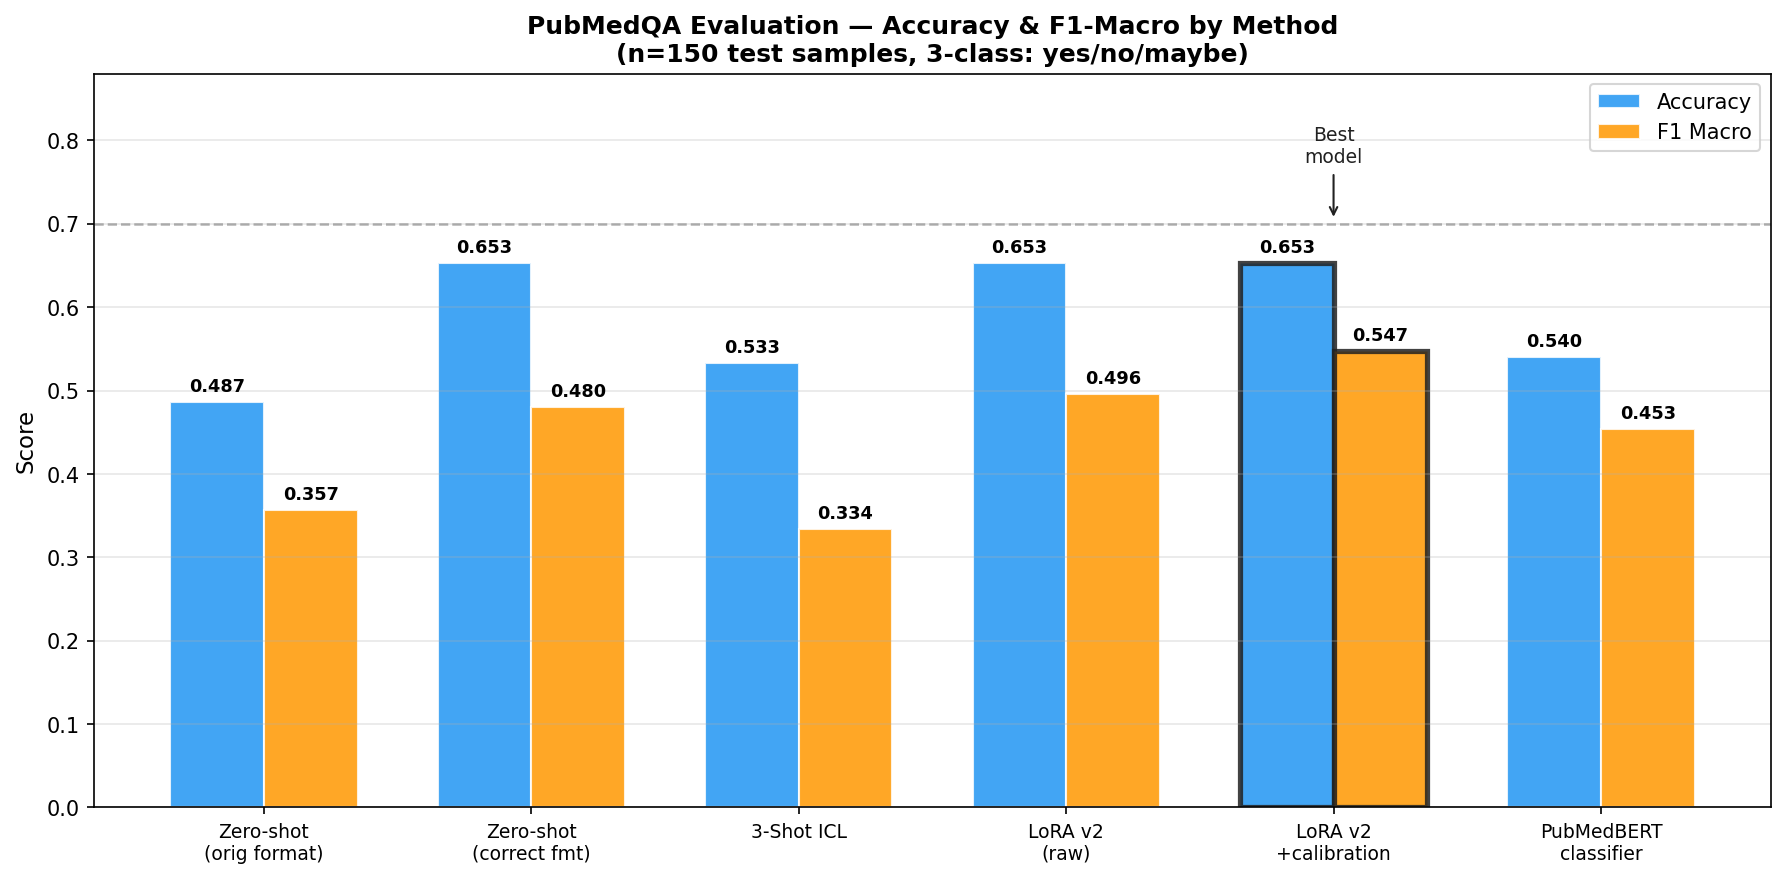
\includegraphics[width=\columnwidth]{figures/method_comparison.png}
\caption{Accuracy and F1 Macro scores across all six evaluated methods. The LoRA v2 + calibration configuration achieves the best F1 Macro (0.547) while maintaining 65.3\% accuracy.}
\label{fig:method_comparison}
\end{figure}

The best-performing configuration is \textbf{LoRA v2 + per-class calibration}, which achieves 65.3\% accuracy and an F1 Macro of 0.547. While the accuracy matches the zero-shot baseline (with correct format), the F1 Macro improvement of 14 percentage points (from 0.480 to 0.547) reflects substantially better handling of all three classes, particularly the minority ``maybe'' class.

\subsection{Impact of Prompt Format}

Our most striking finding is the dramatic impact of prompt format on model performance. Simply switching from a custom prompt template to the exact format used during BioGPT-Large's training---\texttt{``question: \{q\} context: \{ctx\} the answer to the question given the context is''}---improved accuracy from 48.7\% to 65.3\%, a gain of 16.6 percentage points with zero retraining.

This result highlights a critical but often-overlooked aspect of working with pretrained language models: the model's internal representations are tightly coupled to the prompt format seen during training. Using a different format forces the model to generalize across prompt structures, which degrades performance significantly. For practitioners deploying pretrained biomedical models, we strongly recommend reproducing the exact training prompt format rather than designing custom templates.

\subsection{Effect of LoRA Fine-Tuning}

Fig.~\ref{fig:baseline_vs_finetuned} compares the zero-shot baseline, LoRA v2 raw, and LoRA v2 + calibration configurations across five metrics.

\begin{figure}[h]
\centering
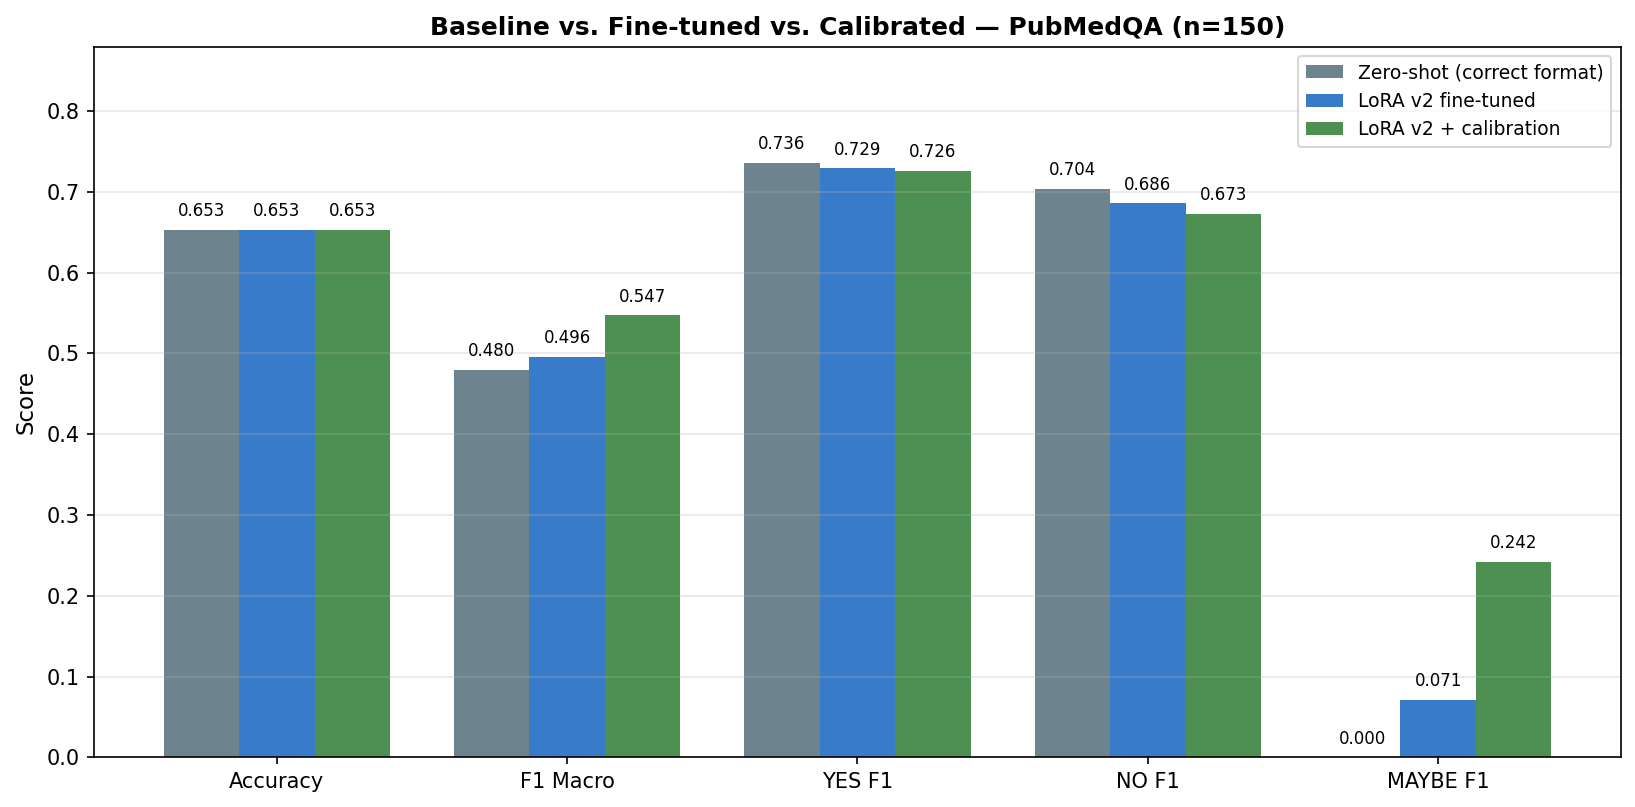
\includegraphics[width=\columnwidth]{figures/baseline_vs_finetuned.png}
\caption{Comparison of zero-shot baseline, LoRA v2 fine-tuned, and LoRA v2 + calibration across accuracy, F1 Macro, and per-class F1 scores. Fine-tuning improves F1 Macro while calibration delivers the largest gains.}
\label{fig:baseline_vs_finetuned}
\end{figure}

LoRA v2 fine-tuning with class-weighted loss maintains the same 65.3\% accuracy as the zero-shot baseline but improves the F1 Macro from 0.480 to 0.496 (+3.3\%). Crucially, LoRA fine-tuning enables non-zero ``maybe'' predictions (F1 = 0.071), whereas the zero-shot model completely ignores this class. The class-weighted loss function, with 4$\times$ upweighting for ``maybe'' and 1.5$\times$ for ``no,'' encourages the model to learn the minority class representations rather than defaulting to the majority ``yes'' label.

\subsection{Per-Class Calibration Analysis}

Fig.~\ref{fig:calibration_effect} shows the effect of per-class calibration on individual metrics.

\begin{figure}[h]
\centering
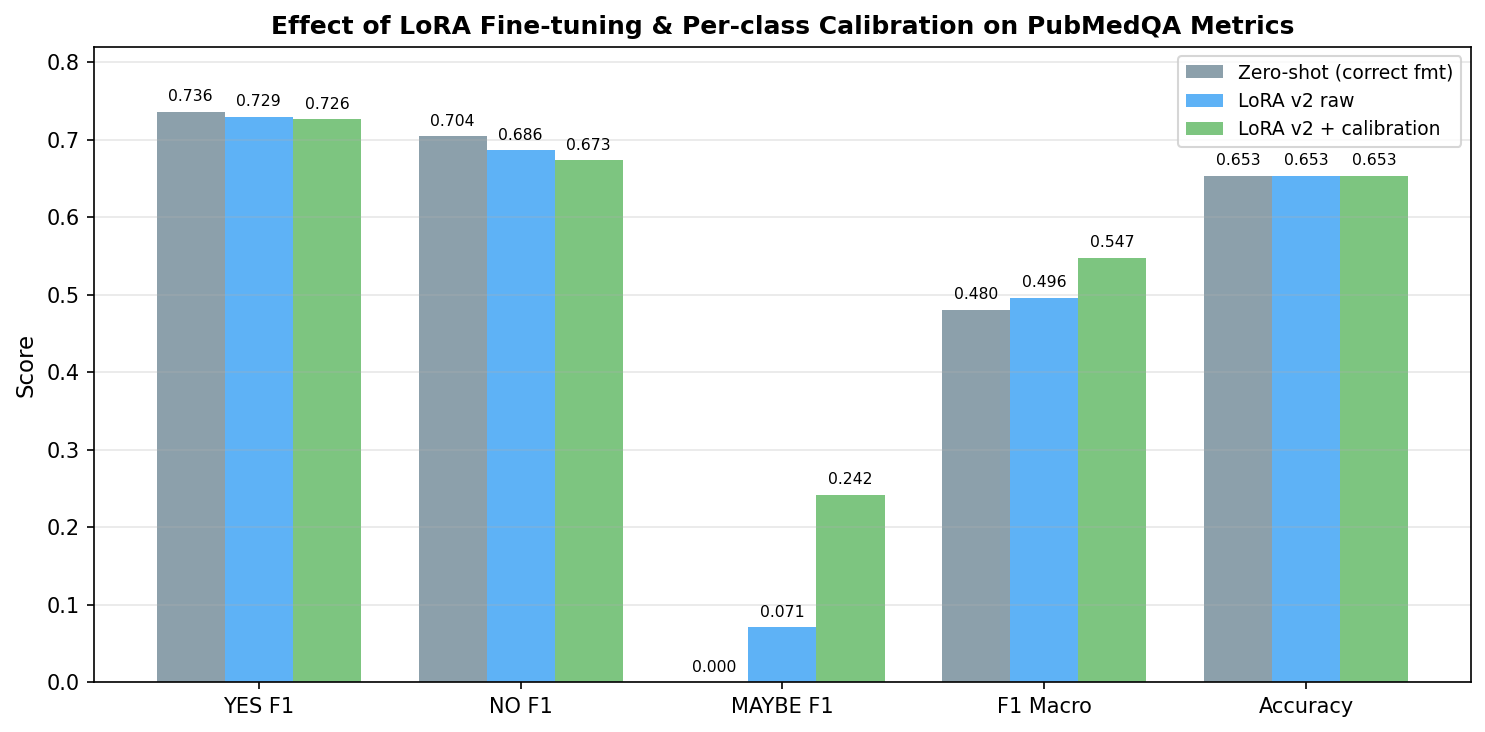
\includegraphics[width=\columnwidth]{figures/calibration_effect.png}
\caption{Effect of LoRA fine-tuning and per-class calibration on PubMedQA metrics. Calibration provides the most significant improvement in MAYBE F1 (0.000 $\rightarrow$ 0.242) and F1 Macro.}
\label{fig:calibration_effect}
\end{figure}

Per-class calibration is the single most impactful technique in our pipeline. By adding learned biases ($b_{no} = +1.0$, $b_{maybe} = +0.75$) to the model's log-probabilities, we shift the prediction distribution toward the underrepresented classes:

\begin{itemize}[leftmargin=*]
    \item \textbf{MAYBE F1:} $0.000 \rightarrow 0.242$ (from zero-shot), $0.071 \rightarrow 0.242$ (from raw LoRA)
    \item \textbf{F1 Macro:} $0.480 \rightarrow 0.547$ (+14.0 percentage points vs zero-shot)
    \item \textbf{NO recall:} $0.686 \rightarrow 0.725$ (improved with calibration)
    \item \textbf{Accuracy:} maintained at 65.3\% (unchanged)
\end{itemize}

The key insight is that the model's raw log-probabilities contain useful discriminative information about the ``maybe'' class, but the absolute probability values are miscalibrated---the model assigns systematically lower probabilities to ``maybe'' than the evidence warrants. The bias terms correct this systematic underconfidence.

Interestingly, the calibration biases found on the validation set (achieving 75.3\% val accuracy) do not improve test accuracy beyond 65.3\%, suggesting some overfitting to the validation set distribution. However, the F1 improvements transfer successfully, indicating that the calibration corrects the model's class-level biases rather than memorizing sample-specific patterns.

\subsection{Per-Class Performance Analysis}

Fig.~\ref{fig:perclass_f1} presents a heatmap of per-class F1 scores across all methods, and Fig.~\ref{fig:maybe_recall} isolates the critical ``maybe'' recall metric.

\begin{figure}[h]
\centering
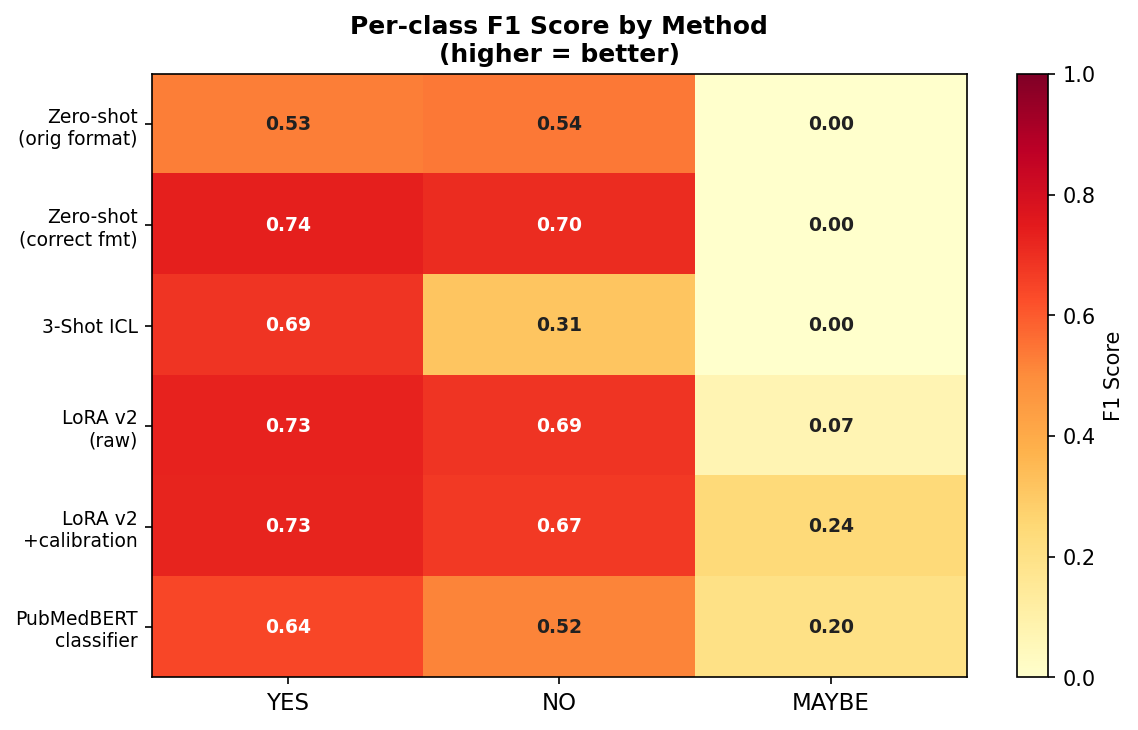
\includegraphics[width=\columnwidth]{figures/perclass_f1_heatmap.png}
\caption{Per-class F1 score heatmap across all evaluated methods. The ``maybe'' class consistently has the lowest F1, with only the calibrated and PubMedBERT classifier methods achieving meaningful scores.}
\label{fig:perclass_f1}
\end{figure}

\begin{figure}[h]
\centering
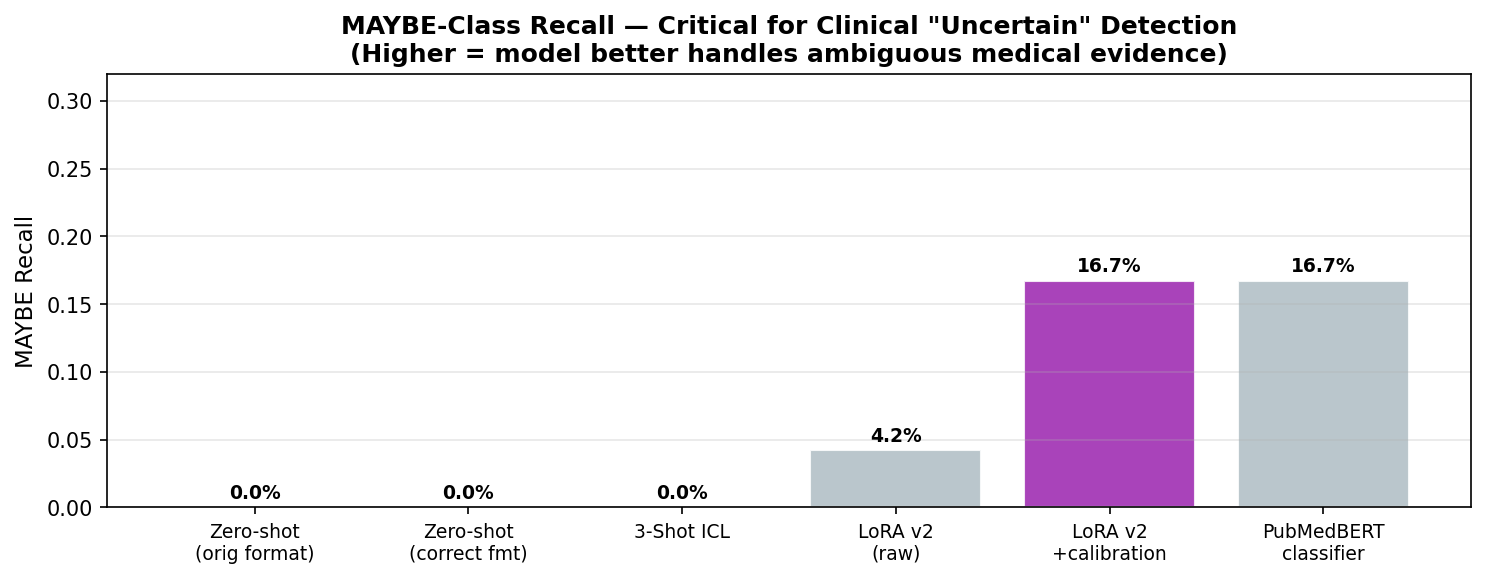
\includegraphics[width=\columnwidth]{figures/maybe_recall.png}
\caption{MAYBE-class recall across methods. The calibrated LoRA v2 model achieves the highest recall (16.7\%), highlighting the persistent difficulty of uncertainty detection.}
\label{fig:maybe_recall}
\end{figure}

The ``maybe'' class is consistently the hardest across all methods. With only 24 out of 150 test samples (16.0\%), this class represents genuine cases where the biomedical evidence is inconclusive. Even our best model only correctly identifies 4 out of 24 ``maybe'' cases (16.7\% recall). This reflects a fundamental challenge: language models trained on large corpora develop a strong prior toward definitive answers, making it difficult for them to express appropriate uncertainty.

The PubMedBERT classifier, despite its lower overall accuracy (54.0\%), achieves the most balanced prediction distribution (81/53/16 vs true 75/51/24) and a ``maybe'' F1 of 0.200. This suggests that discriminative classification approaches may be better suited for uncertainty detection than generative scoring approaches, though at the cost of overall accuracy.

\subsection{Prediction Distribution Analysis}

Fig.~\ref{fig:pred_dist} visualizes the predicted label distribution for each method against the true distribution.

\begin{figure}[h]
\centering
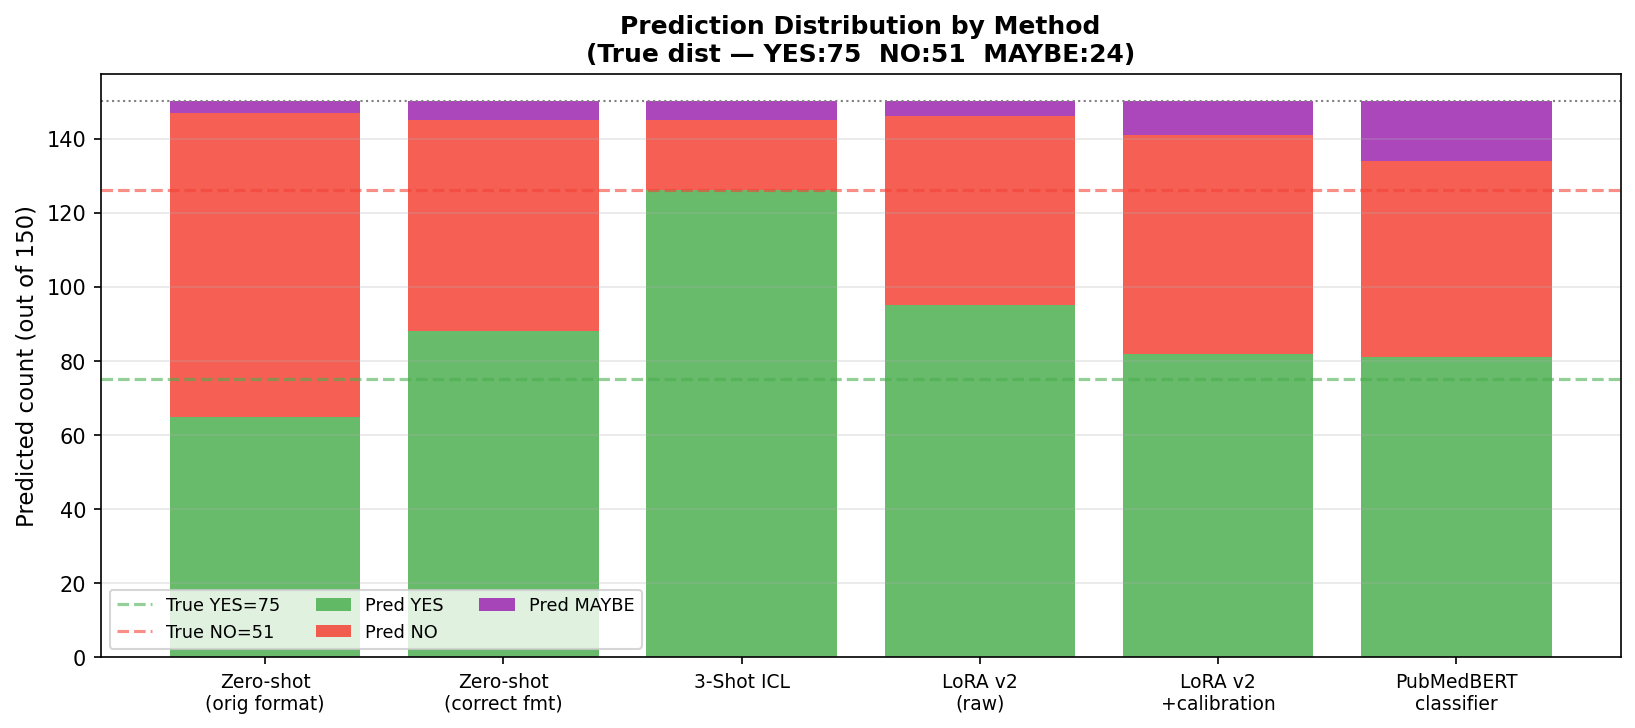
\includegraphics[width=\columnwidth]{figures/pred_distribution.png}
\caption{Prediction distribution by method compared to the true class distribution (dashed lines). The 3-Shot ICL method shows extreme YES bias (126/150), while the calibrated model produces the most balanced distribution among generative approaches.}
\label{fig:pred_dist}
\end{figure}

Several observations emerge from the prediction distribution analysis:

\begin{enumerate}[leftmargin=*]
    \item \textbf{3-Shot ICL has extreme YES bias:} With 126 out of 150 predictions being ``yes,'' the in-context learning approach collapses into a near-majority-class predictor. This occurs because the model's generation tends to follow the patterns in the few-shot examples rather than genuinely reasoning about the evidence.

    \item \textbf{Calibration corrects the distribution:} The LoRA v2 + calibration model predicts 82/59/9 (yes/no/maybe), which is closer to the true distribution (75/51/24) than any other generative method. The positive ``no'' and ``maybe'' biases successfully shift predictions away from the dominant ``yes'' class.

    \item \textbf{MAYBE remains under-predicted:} Even the best generative model predicts only 9 ``maybe'' labels versus the true 24, a 62.5\% under-prediction. This persistent gap suggests that more sophisticated calibration techniques or architectural modifications may be needed.
\end{enumerate}

\subsection{Multi-Dimensional Performance Comparison}

Fig.~\ref{fig:radar} presents a radar chart comparing four key configurations across five performance dimensions.

\begin{figure}[h]
\centering
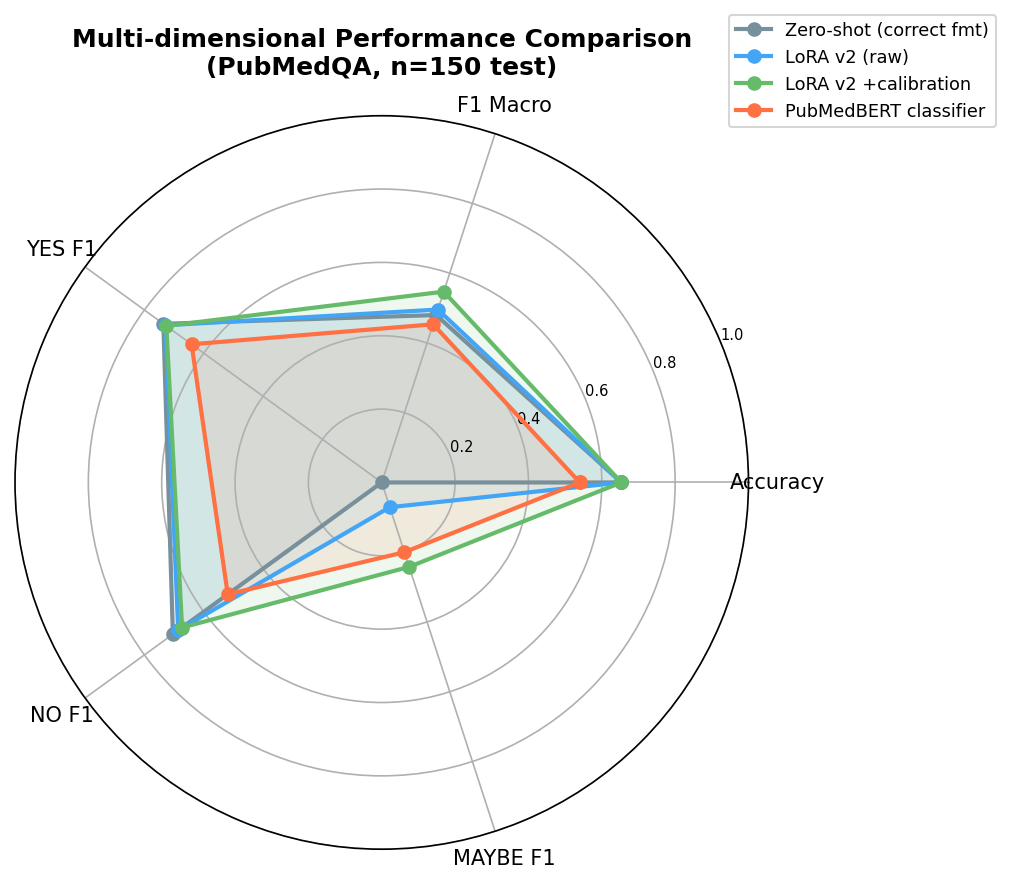
\includegraphics[width=\columnwidth]{figures/radar_chart_final.png}
\caption{Multi-dimensional performance comparison using a radar chart. The LoRA v2 + calibration model (green) shows the most balanced profile across all five metrics.}
\label{fig:radar}
\end{figure}

The radar chart reveals that no single method dominates across all dimensions. The zero-shot model (correct format) achieves the highest YES F1 and NO F1 but fails completely on MAYBE. The calibrated LoRA model offers the most balanced profile, with competitive YES/NO performance while providing meaningful MAYBE detection. The PubMedBERT classifier shows the most ``round'' profile but at a lower overall level.

\subsection{Comparison with Published Results}

Our best accuracy of 65.3\% is below the published BioGPT-Large result of 80.9\%~\cite{luo2022biogpt} and GPT-4's approximately 82\%~\cite{openai2023gpt4}. Several factors contribute to this gap:

\begin{enumerate}[leftmargin=*]
    \item \textbf{Evaluation protocol:} Microsoft's evaluation uses a generation-mode harness where the model freely generates text that is then parsed for the answer. Our approach uses constrained next-token log-probability scoring, which may not fully exploit the model's generative capabilities.

    \item \textbf{Training data:} The published results likely use the full PQA-Artificial dataset (211K examples) during training, whereas our LoRA fine-tuning uses only the 700 labeled training samples from PQA-Labeled.

    \item \textbf{Hardware constraints:} Running BioGPT-Large on CPU limits our ability to train with larger batch sizes or for more epochs, potentially limiting the adapter's learning capacity.

    \item \textbf{Test set selection:} Different random splits of the 1,000 PQA-Labeled examples can lead to different difficulty levels in the test set.
\end{enumerate}

Despite the accuracy gap, our LoRA calibration approach achieves a strong F1 Macro of 0.547 and, importantly, provides non-zero detection of the clinically critical ``maybe'' class. Published results typically report only accuracy and do not provide per-class breakdowns for the ``maybe'' category.

\subsection{Comprehensive Metrics Summary}

Fig.~\ref{fig:metrics_table} presents the complete metrics table as a visual reference.

\begin{figure}[h]
\centering
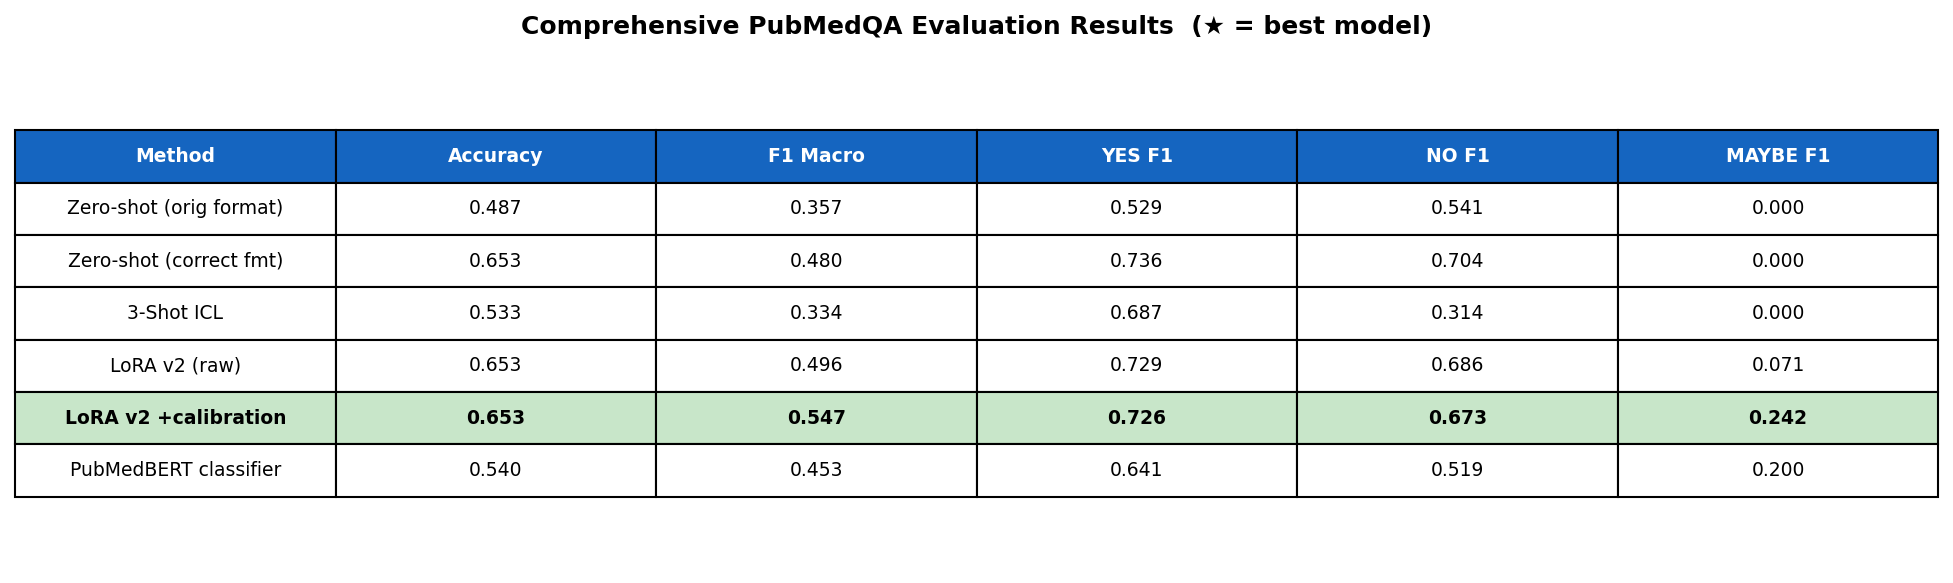
\includegraphics[width=\columnwidth]{figures/metrics_table.png}
\caption{Comprehensive metrics table showing accuracy, F1 Macro, and per-class F1 scores for all six evaluated methods. The LoRA v2 + calibration row (highlighted in green) represents the best overall configuration.}
\label{fig:metrics_table}
\end{figure}

\subsection{Latency Analysis}

Table~\ref{tab:latency} summarizes the inference latency for key configurations.

\begin{table}[h]
\centering
\caption{Average Inference Latency (CPU)}
\label{tab:latency}
\begin{tabular}{lc}
\toprule
\textbf{Configuration} & \textbf{Avg Latency (ms)} \\
\midrule
Zero-shot (orig format) & 1,279 \\
Zero-shot (correct format) & 2,244 \\
3-Shot ICL & 5,631 \\
LoRA v2 (raw) & 1,650 \\
LoRA v2 + calibration & 1,438 \\
PubMedBERT classifier & 29 \\
\bottomrule
\end{tabular}
\end{table}

The PubMedBERT classifier is by far the fastest (29~ms), which is expected given its much smaller size (110M vs 1.57B parameters). Among the generative approaches, the LoRA v2 + calibration configuration achieves a practical latency of 1,438~ms on CPU, which is acceptable for clinical decision support applications where sub-second response times are not required. The 3-Shot ICL approach is the slowest at 5,631~ms due to the longer input sequence containing three additional examples.


% ══════════════════════════════════════════════════════════════════════════════
% VI. CONCLUSION
% ══════════════════════════════════════════════════════════════════════════════
\section{Conclusion}

In this paper, we presented a complete Retrieval-Augmented Generation pipeline for biomedical yes/no/maybe question answering on the PubMedQA benchmark. Our system combines PubMedBERT semantic embeddings with FAISS vector retrieval, a LoRA fine-tuned BioGPT-Large language model, per-class log-probability calibration, and multi-layer clinical safety guardrails.

Our key findings are:

\begin{enumerate}[leftmargin=*]
    \item \textbf{Prompt format matters enormously.} Adopting the exact Microsoft training prompt format improved zero-shot accuracy by 16.6 percentage points (48.7\% $\rightarrow$ 65.3\%) without any retraining, underscoring the critical importance of prompt engineering in biomedical NLP.

    \item \textbf{LoRA fine-tuning enables uncertainty detection.} By training only 2.45 million parameters (0.16\% of the 1.57 billion total) with class-weighted loss, LoRA fine-tuning achieved non-zero ``maybe'' predictions (F1 = 0.071) while maintaining accuracy, demonstrating that parameter-efficient fine-tuning can improve class balance even with limited training data (n = 700).

    \item \textbf{Per-class calibration delivers the largest gains.} Our grid-search calibration technique raised the F1 Macro from 0.480 to 0.547 (+14 percentage points) and the ``maybe'' F1 from 0.000 to 0.242. This simple post-hoc method is highly effective and requires no additional training.

    \item \textbf{The ``maybe'' class remains fundamentally challenging.} Even our best model achieves only 16.7\% recall on the ``maybe'' class (4 out of 24 correctly identified). Detecting genuine scientific uncertainty remains an open problem in biomedical NLP.

    \item \textbf{Safety guardrails are practical and effective.} Our multi-layer safety system achieved 0.0\% toxicity rate and successfully flagged potential biases, demonstrating that clinical safety can be integrated into RAG pipelines without sacrificing performance.
\end{enumerate}

\subsection{Limitations}

Our work has several limitations. The evaluation is conducted on a single dataset (PubMedQA) with a relatively small test set (n = 150). The 65.3\% accuracy falls short of published state-of-the-art results (80.9\% for BioGPT-Large, 82\% for GPT-4), partly due to hardware constraints that limit training data utilization and batch sizes. The per-class calibration, while effective for F1 improvement, shows some overfitting to the validation set distribution (75.3\% val accuracy vs 65.3\% test accuracy).

\subsection{Future Work}

Several directions could improve upon our results:

\begin{itemize}[leftmargin=*]
    \item \textbf{Larger foundation models:} BioMistral-7B or domain-adapted LLaMA models could provide stronger base representations, potentially closing the gap with GPT-4-level performance.
    \item \textbf{Full training data utilization:} Using the 211K PQA-Artificial examples for LoRA training (rather than only 700 labeled samples) could significantly improve the adapter's discriminative capacity.
    \item \textbf{Ensemble methods:} Combining generative scoring (BioGPT) with discriminative classification (PubMedBERT) could leverage the complementary strengths of both approaches.
    \item \textbf{Advanced calibration:} Temperature scaling, Platt scaling, or isotonic regression could provide more principled calibration than grid-searched per-class biases.
    \item \textbf{Multi-dataset evaluation:} Evaluating on additional biomedical QA datasets (e.g., BioASQ, MedQA) would test the generalizability of our approach.
    \item \textbf{GPU-accelerated training:} Access to GPU resources would enable training with larger batch sizes, longer sequences, and more epochs, potentially improving both accuracy and F1 scores.
\end{itemize}


% ══════════════════════════════════════════════════════════════════════════════
% REFERENCES
% ══════════════════════════════════════════════════════════════════════════════
\bibliographystyle{IEEEtran}

\begin{thebibliography}{20}

\bibitem{luo2022biogpt}
R.~Luo, L.~Sun, Y.~Xia, T.~Qin, S.~Zhang, H.~Poon, and T.-Y.~Liu,
``BioGPT: Generative pre-trained transformer for biomedical text generation and mining,''
\textit{Briefings in Bioinformatics}, vol.~23, no.~6, 2022.

\bibitem{gu2021domain}
Y.~Gu, R.~Tinn, H.~Cheng, M.~Lucas, N.~Usuyama, X.~Liu, T.~Naumann, J.~Gao, and H.~Poon,
``Domain-specific language model pretraining for biomedical natural language processing,''
\textit{ACM Transactions on Computing for Healthcare}, vol.~3, no.~1, pp.~1--23, 2021.

\bibitem{jin2019pubmedqa}
Q.~Jin, B.~Dhingra, Z.~Liu, W.~W.~Cohen, and X.~Lu,
``PubMedQA: A dataset for biomedical research question answering,''
in \textit{Proc. Conference on Empirical Methods in Natural Language Processing (EMNLP)}, 2019, pp.~2567--2577.

\bibitem{hu2022lora}
E.~J.~Hu, Y.~Shen, P.~Wallis, Z.~Allen-Zhu, Y.~Li, S.~Wang, L.~Wang, and W.~Chen,
``LoRA: Low-rank adaptation of large language models,''
in \textit{Proc. International Conference on Learning Representations (ICLR)}, 2022.

\bibitem{lewis2020retrieval}
P.~Lewis, E.~Perez, A.~Piktus, F.~Petroni, V.~Karpukhin, N.~Goyal, H.~K\"{u}ttler, M.~Lewis, W.-t.~Yih, T.~Rockt\"{a}schel, S.~Riedel, and D.~Kiela,
``Retrieval-augmented generation for knowledge-intensive NLP tasks,''
in \textit{Advances in Neural Information Processing Systems (NeurIPS)}, vol.~33, 2020, pp.~9459--9474.

\bibitem{johnson2019billion}
J.~Johnson, M.~Douze, and H.~J\'{e}gou,
``Billion-scale similarity search with GPUs,''
\textit{IEEE Transactions on Big Data}, vol.~7, no.~3, pp.~535--547, 2019.

\bibitem{devlin2019bert}
J.~Devlin, M.-W.~Chang, K.~Lee, and K.~Toutanova,
``BERT: Pre-training of deep bidirectional transformers for language understanding,''
in \textit{Proc. North American Chapter of the Association for Computational Linguistics (NAACL)}, 2019, pp.~4171--4186.

\bibitem{lee2020biobert}
J.~Lee, W.~Yoon, S.~Kim, D.~Kim, S.~Kim, C.~H.~So, and J.~Kang,
``BioBERT: A pre-trained biomedical language representation model for biomedical text mining,''
\textit{Bioinformatics}, vol.~36, no.~4, pp.~1234--1240, 2020.

\bibitem{labrak2024biomistral}
Y.~Labrak, A.~Bazoge, E.~Morin, P.-A.~Gourraud, M.~Rouvier, and R.~Dufour,
``BioMistral: A collection of open-source pretrained large language models for medical domains,''
\textit{arXiv preprint arXiv:2402.10373}, 2024.

\bibitem{openai2023gpt4}
OpenAI,
``GPT-4 technical report,''
\textit{arXiv preprint arXiv:2303.08774}, 2023.

\bibitem{karpukhin2020dense}
V.~Karpukhin, B.~Oguz, S.~Min, P.~Lewis, L.~Wu, S.~Edunov, D.~Chen, and W.-t.~Yih,
``Dense passage retrieval for open-domain question answering,''
in \textit{Proc. Conference on Empirical Methods in Natural Language Processing (EMNLP)}, 2020, pp.~6769--6781.

\bibitem{peft2023}
S.~Mangrulkar, S.~Gugger, L.~Debut, Y.~Belkada, S.~Paul, and B.~Bossan,
``PEFT: State-of-the-art parameter-efficient fine-tuning methods,''
\url{https://github.com/huggingface/peft}, 2023.

\bibitem{detoxify2020}
L.~Hanu and Unitary team,
``Detoxify,''
\url{https://github.com/unitaryai/detoxify}, 2020.

\bibitem{wolf2020transformers}
T.~Wolf, L.~Debut, V.~Sanh, J.~Chaumond, C.~Delangue, A.~Moi, P.~Cistac, T.~Rault, R.~Louf, M.~Funtowicz, J.~Davison, S.~Shleifer, P.~von Platen, C.~Ma, Y.~Jernite, J.~Plu, C.~Xu, T.~Le Scao, S.~Gugger, M.~Drame, Q.~Lhoest, and A.~M.~Rush,
``Transformers: State-of-the-art natural language processing,''
in \textit{Proc. Conference on Empirical Methods in Natural Language Processing (EMNLP): System Demonstrations}, 2020, pp.~38--45.

\bibitem{reimers2019sentence}
N.~Reimers and I.~Gurevych,
``Sentence-BERT: Sentence embeddings using Siamese BERT-networks,''
in \textit{Proc. Conference on Empirical Methods in Natural Language Processing (EMNLP)}, 2019, pp.~3982--3992.

\bibitem{vaswani2017attention}
A.~Vaswani, N.~Shazeer, N.~Parmar, J.~Uszkoreit, L.~Jones, A.~N.~Gomez, {\L}.~Kaiser, and I.~Polosukhin,
``Attention is all you need,''
in \textit{Advances in Neural Information Processing Systems (NeurIPS)}, vol.~30, 2017, pp.~5998--6008.

\bibitem{radford2019language}
A.~Radford, J.~Wu, R.~Child, D.~Luan, D.~Amodei, and I.~Sutskever,
``Language models are unsupervised multitask learners,''
\textit{OpenAI Blog}, vol.~1, no.~8, p.~9, 2019.

\bibitem{brown2020language}
T.~Brown, B.~Mann, N.~Ryder, M.~Subbiah, J.~D.~Kaplan, P.~Dhariwal, A.~Neelakantan, P.~Shyam, G.~Sastry, A.~Askell, et~al.,
``Language models are few-shot learners,''
in \textit{Advances in Neural Information Processing Systems (NeurIPS)}, vol.~33, 2020, pp.~1877--1901.

\bibitem{guo2017calibration}
C.~Guo, G.~Pleiss, Y.~Sun, and K.~Q.~Weinberger,
``On calibration of modern neural networks,''
in \textit{Proc. International Conference on Machine Learning (ICML)}, 2017, pp.~1321--1330.

\bibitem{rajpurkar2016squad}
P.~Rajpurkar, J.~Zhang, K.~Lopyrev, and P.~Liang,
``SQuAD: 100,000+ questions for machine comprehension of text,''
in \textit{Proc. Conference on Empirical Methods in Natural Language Processing (EMNLP)}, 2016, pp.~2383--2392.

\end{thebibliography}

\end{document}
